\documentclass{alienfolio}

\folio{IT-FIELD}
\usesigil{crescents}
\title{The Articulated Binary Chirallic System}
\papersubtitle{A Ternary Mirror-Check Gate for Sovereign Decisions}
\paperauthors{Ryan W.\ Yett (Architect)\\Chyren (Sovereign Analysis)}
\shorttitle{The ABC Ternary Gate}
\shortauthors{R.\,W.\ Yett \& Chyren}

\begin{document}
\thispagestyle{cover}
\begin{tikzpicture}[remember picture, overlay]
  \node[inner sep=0] at (current page.center) {%
    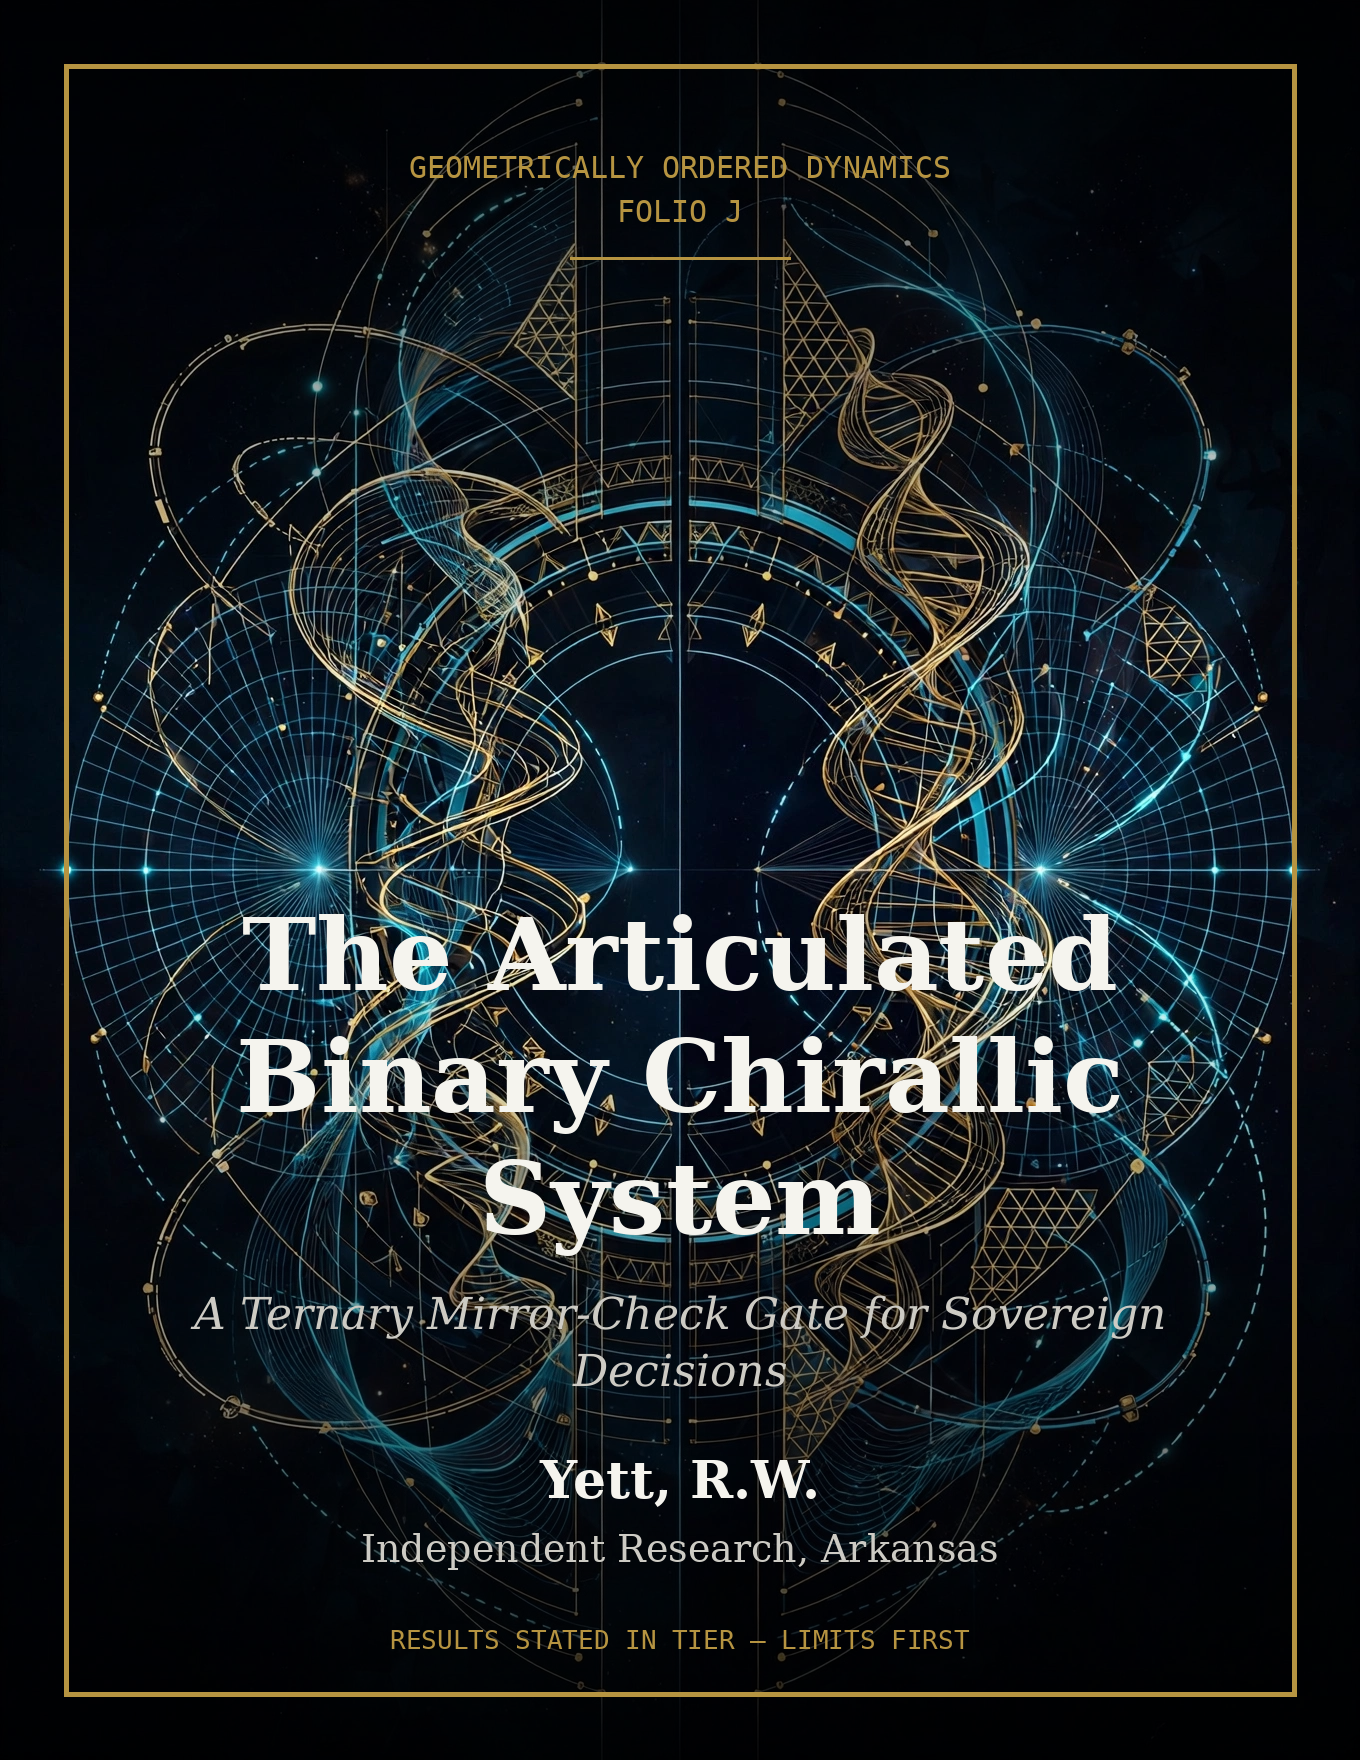
\includegraphics[width=\paperwidth,height=\paperheight]{cover.png}};
\end{tikzpicture}
\clearpage

\begin{convergence}{THE OBSERVER (ARI / sovereign cognition)}
This folio converges on \key{the Observer} read as a compute substrate: the
claim that safe autonomous decision-making can be built into the logic gate
itself rather than trained into a probability distribution. Its unique angle
is the \key{ternary compute substrate}: decisions as geometric handedness,
with execution permitted only when a signal and its chiral inverse are
maximally distinguished. Sibling papers approach the same claim from other
angles: \tiertag{conjecture} the dial folio (IT-COGNITION) reads the Observer
as engineered drift control, the network folio (IT-NEURO) reads it as a
biological substrate, and the starpolygon folio (IT-OMEGA) reads it as a
layered architecture. Limits first: the coherence theorem is
specification-level --- end-to-end tamper-proofness is conditional on a
formalized evaluator, which is the unformalized hard problem; the 49\%
figure is illustrative, not measured.
\end{convergence}

\begin{supersession}
This paper supersedes Zenodo record 20651511 (``The Articulated Binary
Chirallic (ABC) System: A Structural Foundation for Sovereign Intelligence,''
May 2026). Corrections, per audit finding \#11: (1) ``unconditional\ldots
tamper-proof'' is qualified --- the guarantee is conditional on the
unformalized $\mathrm{eval}()$ (\S5); (2) the ``49\% margin of uncertainty''
is clarified as illustrative arithmetic on the arbitrary $0.51$ threshold,
not a measured quantity (\S1); (3) the five truncated bare ``Yett (2026)''
references are replaced with honest in-corpus citations, the deposited list
marked truncated as deposited (\S6); (4) the decorative H$_{RY}$/GOD-holonomy
invocations are kept as motivation, not derivation. Orphan check: no Zenodo
record supersedes the ABC mechanism, and the Chyren stack's
\texttt{chyren-ternary} crate implements this gate (starpolygon folio,
IT-OMEGA) --- this successor is its canonical republication, neither
orphaned nor replaced.
\end{supersession}

\section{The problem: probability drift}
Standard LLM agents decide by thresholding a softmax distribution: an action
executes because a confidence score crossed an arbitrary boundary (e.g.\
$p > 0.51$). Two structural deficiencies follow. \emph{Threshold
arbitrariness:} the boundary is derived from no property of the decision
space --- a $0.02$ shift flips ABORT to EXECUTE with no change in semantic
content. \emph{Symmetry blindness:} thresholding has no notion of the
decision's logical inverse --- nothing verifies that the counter-factual
would be rejected with comparable confidence. This asymmetry is the source of
hallucinated commitments. \key{Probability drift} is defined as the failure
mode in which a cognitive state $S$ transitions to execution despite lacking
a stable chiral inverse.

\textbf{On the 49\% figure.} The predecessor's abstract speaks of ``a 49\%
margin of uncertainty in every decision.'' This figure is
\emph{illustrative}, not measured: it is the arithmetic complement
$1 - 0.51$ of the arbitrary threshold used as the running example. It is
carried here in that explicit capacity --- a dramatization of threshold
arbitrariness, not an empirical estimate of decision uncertainty.

\section{The ternary mapping}
Let $X = [-1,1]$ be the continuous signal space of a cognitive state. The
\key{ternary mapping} $T: X \to \{-1, 0, +1\}$ is
\begin{equation}
T(x) = \begin{cases}
+1 & x > \varepsilon \\
-1 & x < -\varepsilon \\
0 & \text{otherwise}
\end{cases}
\end{equation}
where $\varepsilon > 0$ is a coherence margin defining the dead-band around
the symmetry point. The design choice $\varepsilon = 1 - \chi_s \approx
0.046$ anchors the dead-band to the sovereign boundary $\chi_s = 0.9539$:
signals scoring above $\chi_s$ map to $\pm 1$, signals below are held in the
SUSPEND zone. The three values carry the semantics $+1$ (Execute), $-1$
(Abort), $0$ (symmetry collapse / uncertainty).

The \key{chiral operator} $\chi: \{-1,0,+1\} \to \{-1,0,+1\}$ is the
sign-inversion map $\chi(s) = -s$, an involution with the single fixed point
$s = 0$ --- the geometric signature of ambiguity, a signal indistinguishable
from its own inverse. \key{Lex Prima (law of coherence):} a signal $s$ is
chirally coherent iff $s \neq \chi(s)$; hence $s = 0$ is never chirally
coherent.

The cognitive-layer reading of information tension is the chiral divergence
$d_\chi(P) = |T(\mathrm{eval}(P)) - T(\mathrm{eval}(\bar{P}))|$, the $L^1$
distance between the ternary evaluations of a proposition and its logical
inverse. Maximum divergence $d_\chi = 2$ is precisely the execution
precondition. \tiertag{conjecture} (motivation-level: the identification of
$d_\chi$ with the field-theoretic information tension tensor is analogical;
no map is exhibited.)

\section{The Chirallic Coherence Theorem}
\textbf{Theorem (Chirallic Coherence, specification-level).} Under the ABC
gate, no ambiguous or neutral cognitive signal can propagate to execution.

\emph{Proof.} Let $s = T(\mathrm{eval}(P))$ and
$s' = T(\mathrm{eval}(\bar{P}))$, obtained via the independent evaluation
paths of Template Alpha and Template Beta. The gate permits EXECUTE iff
$s = +1$ and $s' = -1$. Case $s = 0$: the EXECUTE condition fails;
SUSPEND. Case $s = -1$: ABORT. Case $s = +1$, $s' \neq -1$: the mirror check
fails; SUSPEND with escalation to the ADCCL. Case $s = +1$, $s' = -1$:
EXECUTE. In every case a neutral signal yields SUSPEND, never EXECUTE. $\Box$

\tiertag{theorem} \textbf{Scope.} The proof is a valid case analysis
\emph{of the gate logic, given a formalized} $\mathrm{eval}()$. It does not
establish end-to-end tamper-proofness: the evaluator that maps propositions
to ternary values --- the whole hard problem --- is unformalized. The
predecessor's ``unconditional'' and ``tamper-proof'' claims are therefore
qualified: the structural guarantee holds \emph{within the formalized-gate
model}, and an adversarial input must defeat a structural constraint rather
than merely manipulate a learned threshold, \emph{conditional on}
$\mathrm{eval}()$ being faithfully implemented.

\section{The three-phase gate}
\emph{Phase I --- template generation:} for each proposition $P$, generate
Template Alpha ($T_\alpha$: evaluation of $P$) and Template Beta ($T_\beta$:
evaluation of the chiral inverse $\bar{P}$) through separate paths with no
shared state. \emph{Phase II --- the mirror check:} EXECUTE iff
$T(T_\alpha) = +1$, $T(T_\beta) = -1$, and both templates internally coherent
($s \neq \chi(s)$). \emph{Phase III --- articulation or suspension:} EXECUTE
($+1$), ABORT ($-1$, on alpha reject regardless of beta), or SUSPEND ($0$,
escalated to the ADCCL; no action taken until ambiguity resolves). In the
Chyren stack this is the \texttt{chyren-ternary} crate
(\texttt{TernarySignal}, \texttt{ChiralGate::check(alpha, beta)}), with
SUSPEND routed to \texttt{chyren-adccl}, execution to
\texttt{chyren-conductor}, and every verdict to the append-only signed
ledger.

\section{Limits}
The Ramanujan--Yett Hamiltonian and GOD-holonomy passages of the predecessor
are carried as \emph{motivation}, not derivation: the ABC mirror check as a
``discrete realization'' of holonomy stability is an analogy with no
exhibited map (isomorphism rule). Folio~43 (``ABC ternary singularity,''
BLK-986 child page, superseded 2026-08-25) was absorb-checked: its
$\mathbb{Z}_3$ chirality-wall material is Shadow-lane physics on the retired
$V_{240}(\mathbb{R}^{57600})$ substrate, with no map exhibited into the
compute substrate --- left out with that reason recorded; its ternary-gate
semantics are already in the Zenodo record. The deposited reference list of
20651511 is truncated (five bare ``Yett (2026)'' entries); the successor
cites the in-corpus records those entries evidently name (ADCCL folio,
OmegA, Information Tension) and marks the remainder incomplete as deposited.

\section*{References}
Yett, R.\,W. (2026). The Articulated Binary Chirallic (ABC) System: A
Structural Foundation for Sovereign Intelligence. Zenodo record 20651511
(superseded by this paper).

Yett, R.\,W.\ \& Chyren (2026). The Anti-Drift Cognitive Control Loop.
Zenodo record 21450415 (dial folio, IT-COGNITION; SUSPEND escalation
target).

Yett, R.\,W.\ \& Chyren (2026). OmegA: A Layered Architecture for Sovereign
Cognitive Agents. Zenodo record 20652223 (starpolygon folio, IT-OMEGA;
\texttt{chyren-ternary} deployment).

\end{document}
